\documentclass{scrartcl}

\usepackage{tikz}

%Construction of the helix -- from French (1929: 157)
%French, T. (1929). A Manual of Engineering Drawing for Students and Draftsmen. New York: McGraw-Hill

\begin{document}
	
	\hspace{-2.5cm}%
	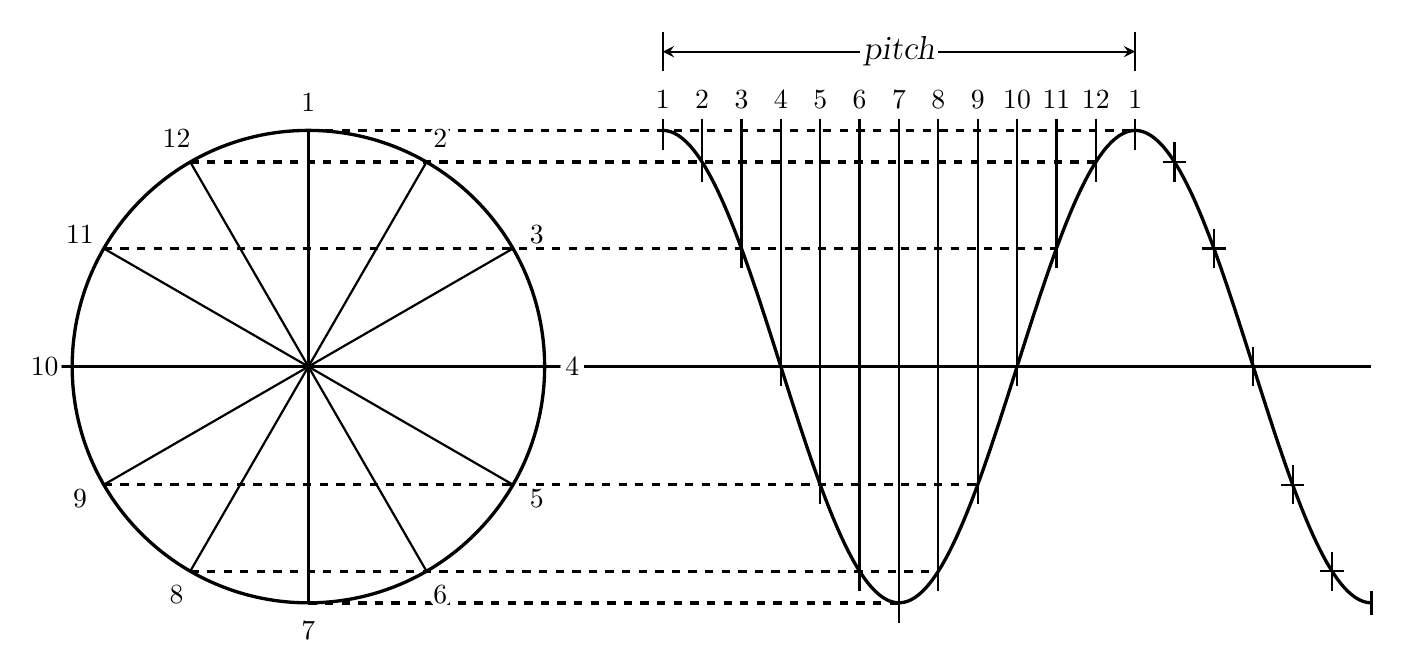
\begin{tikzpicture}
	%CIRCLE
	\draw[very thick] (0,0) circle (3cm);
	\draw[very thick] (-3.15,0)--(13.5,0);	%horizontal axis
	
	%DOTTED LINES
	\foreach \x in {0,...,6} 
	\draw[very thick,dashed] ({3*cos(90+30*\x)}, {3*sin(90+30*\x)}) -- ({4.5+0.5*(12-\x)},{3*sin(90+30*\x)});
	
	%AXELS
	\foreach \x in {1,...,11} 
	\draw[thick] (0,0)--({3*cos(\x*30)},{3*sin(\x*30)});
	%
	\foreach \x in {1,...,12} 	%labels
	\node[circle,draw=white,fill=white,inner sep=0pt,minimum size=5.5pt] at ({3.35*cos(120-\x*30)},{3.35*sin(120-\x*30)}) {\x};
	
	%COSINE CURVE
	\draw[very thick] (4.5,3) cos (6,0) sin (7.5,-3) cos (9,0) sin (10.5,3) cos (12,0) sin (13.5,-3);
	
	%VERTICAL LINES
	\foreach \x in {0,...,6}{
	\draw[thick] (4.5+\x*0.5,3.15)--(4.5+\x*0.5,{3*cos(deg(\x*pi/6))-0.25});	%leftward lines
	\draw[thick] (10.5-\x*0.5,3.15)--(10.5-\x*0.5,{3*cos(deg(\x*pi/6))-0.25});	%rightward lines
	}
	\foreach \x in {1,...,12}	%labels
	\node[align=center,above] at (4+\x*0.5,3.15) {\x};
	\node[align=center,above] at (10.5,3.15) {1};
	%
	\foreach \x in {1,...,5}{	%tics on rightmost part
	\draw[thick] (10.5+\x*0.5,{3*cos(deg(\x*pi/6))+0.25})--(10.5+\x*0.5,{3*cos(deg(\x*pi/6))-0.25}); %|
	\draw[thick] (10.35+\x*0.5,{3*cos(deg(\x*pi/6))})--(10.65+\x*0.5,{3*cos(deg(\x*pi/6))}); %--
	}
	\draw[thick] (13.5,-2.85)--(13.5,-3.15);	%rightmost tic is irregular
	
	%LABELS
	\node at (7.5,4) {\textsl{\large pitch}};
	\draw[thick,->,>=stealth] (7,4)--(4.5,4);	\draw[thick] (4.5,3.75)--(4.5,4.25);
	\draw[thick,->,>=stealth] (8,4)--(10.5,4);	\draw[thick] (10.5,3.75)--(10.5,4.25);
	\end{tikzpicture}
	
\end{document}